\documentclass[border=1pt]{standalone}
\usepackage[dvipsnames]{xcolor}
\usepackage{tikz}                       % Graphen und kommutative Diagramme
\usetikzlibrary{patterns}               % Um schraffierte Formen in der tikzpicture-Umgebung zu zeichnen.
\newcommand{\ul}[1]{\underline{\smash{#1}}}

\begin{document}

\centering
\begin{minipage}{.55\textwidth}
\centering
\resizebox{!}{3cm}{
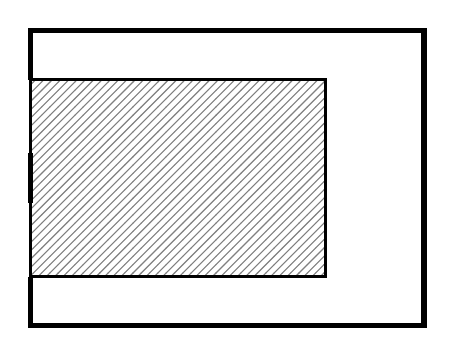
\begin{tikzpicture}[x=1.25cm, y=1.25cm, line width=1pt]
    % draw outer lines
    \draw (0, 0) -- (4, 0) -- (4, 3) -- (0, 3) -- (0, 0);
    
    % draw shaded slit box
    \filldraw[pattern=north east lines, pattern color=black!50] (0, 0.5) -- (3, 0.5) -- (3, 2.5) -- (0, 2.5) -- (0, 0.5);
    
    % draw line width=2pt boundary lines
    \draw[line width=2pt] (0, 0.5) -- (0, 0) -- (4, 0) -- (4, 3) -- (0, 3) -- (0, 2.5);
    \draw[line width=2pt] (0, 1.25) -- (0, 1.75);

\end{tikzpicture}
}
\end{minipage}

\centering
\begin{minipage}{.55\textwidth}
\centering
\resizebox{!}{4.5cm}{
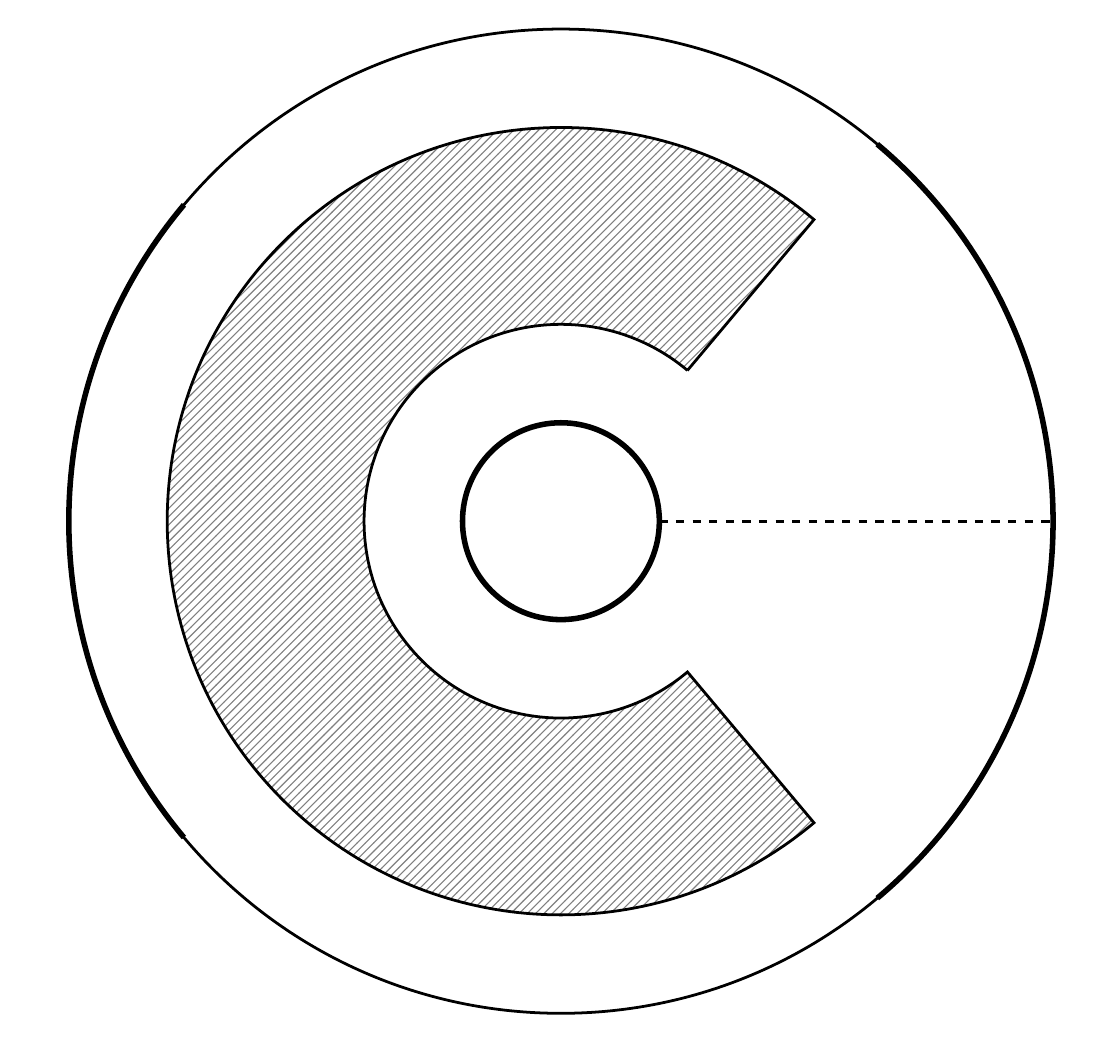
\begin{tikzpicture}[x=1.25cm, y=1.25cm, line width=1pt]
    % draw inner and outer circles
    \draw[color=black] (0, 0) circle (1);
    \draw[color=black] (0, 0) circle (5);
    
    % draw 0 line
    \draw[color=black, dashed] (0 : 1) -- (0 : 5); 
    
    % draw shaded slit box
    \filldraw[pattern=north east lines, pattern color=black!50] 
      (50 : 2) -- (50 : 4) arc [radius = 4, start angle = 50, delta angle = 260] 
	       -- (310 : 2) arc [radius = 2, start angle = 310, delta angle = -260] ;
    
    % draw line width=2pt boundary lines
    \draw[line width=2pt] (0 : 1) arc [radius = 1, start angle = 0, delta angle = 360]; 
    \draw[line width=2pt] (310 : 5) arc [radius = 5, start angle = 310, delta angle = 100]; 
    \draw[line width=2pt] (140 : 5) arc [radius = 5, start angle = 140, delta angle = 80]; 
    
\end{tikzpicture}
}
\end{minipage}


\end{document}
67